\documentclass[12pt, oneside]{book}
\usepackage[a4paper,top=2.5cm,bottom=2.5cm,left=3.5cm,right=2cm]{geometry}
\usepackage[utf8]{inputenc}
\usepackage[T1]{fontenc}
\usepackage{graphicx}
\usepackage{subfig}
\usepackage{url}
\usepackage{enumitem}
\usepackage{makecell}
\usepackage{amsthm}
\usepackage{mathtools}
\usepackage{array}
\usepackage{rotating}
\usepackage{listings,xcolor}
\usepackage[hidelinks,breaklinks]{hyperref}
\usepackage[slovak]{babel} % vypnite pre prace v anglictine
\linespread{1.25} % hodnota 1.25 by mala zodpovedat 1.5 riadkovaniu

% -------------------
% --- Definicia zakladnych pojmov
% --- Vyplnte podla vasho zadania
% -------------------
\def\mfrok{2018}
\def\mfnazov{Inteligentný monitorovací systém práce študentov v Linuxovom termináli}
\def\mftyp{Bakalárska práca}
\def\mfautor{Adrián Matejov}
\def\mfskolitel{RNDr. Marek Nagy, PhD.}

%ak mate konzultanta, odkomentujte aj jeho meno na titulnom liste
\def\mfkonzultant{tit. Meno Priezvisko, tit. }  

\def\mfmiesto{Bratislava, \mfrok}

%aj cislo odboru je povinne a je podla studijneho odboru autora prace
\def\mfodbor{Informatika} 
\def\program{Informatika}
\def\mfpracovisko{Katedra aplikovanej informatiky}

\colorlet{punct}{red!60!black}
\definecolor{delim}{RGB}{20,105,176}
\colorlet{numb}{magenta!60!black}

\lstdefinelanguage{json}{
	basicstyle=\normalfont\ttfamily,
	numbers=left,
	numberstyle=\scriptsize,
	stepnumber=1,
	numbersep=8pt,
	showstringspaces=false,
	breaklines=true,
	frame=lines,
	literate=
	*{0}{{{\color{numb}0}}}{1}
	{1}{{{\color{numb}1}}}{1}
	{2}{{{\color{numb}2}}}{1}
	{3}{{{\color{numb}3}}}{1}
	{4}{{{\color{numb}4}}}{1}
	{5}{{{\color{numb}5}}}{1}
	{6}{{{\color{numb}6}}}{1}
	{7}{{{\color{numb}7}}}{1}
	{8}{{{\color{numb}8}}}{1}
	{9}{{{\color{numb}9}}}{1}
	{:}{{{\color{punct}{:}}}}{1}
	{,}{{{\color{punct}{,}}}}{1}
	{"}{{{\color{delim}{"}}}}{1}
	{\{}{{{\color{delim}{\{}}}}{1}
	{\}}{{{\color{delim}{\}}}}}{1}
	{[}{{{\color{delim}{[}}}}{1}
	{]}{{{\color{delim}{]}}}}{1},
}

\lstdefinelanguage{JavaScript}{
	keywords={typeof, new, true, false, catch, function, return, null, catch, switch, var, if, in, while, do, else, case, break, for},
	keywordstyle=\color{blue}\bfseries,
	ndkeywords={class, export, boolean, throw, implements, import, this},
	ndkeywordstyle=\color{darkgray}\bfseries,
	identifierstyle=\color{black},
	sensitive=false,
	comment=[l]{//},
	morecomment=[s]{/*}{*/},
	commentstyle=\color{purple}\ttfamily,
	stringstyle=\color{red}\ttfamily,
	morestring=[b]',
	morestring=[b]",
	aboveskip=12pt,
}

\lstset{
	language=JavaScript,
	extendedchars=true,
	basicstyle=\small\ttfamily,
	showstringspaces=false,
	showspaces=false,
	frame=single,
	tabsize=2,
	breaklines=true,
	showtabs=true,
	captionpos=b
}

\theoremstyle{definition}
\newtheorem*{prikl}{Príklad}

\newcolumntype{C}[1]{>{\centering\let\newline\\\arraybackslash\hspace{0pt}}m{#1}}
\renewcommand{\thesubfigure}{\arabic{subfigure}}

\begin{document}     
\frontmatter


% -------------------
% --- Obalka ------
% -------------------
\thispagestyle{empty}

\begin{center}
\sc\large
Univerzita Komenského v Bratislave\\
Fakulta matematiky, fyziky a informatiky

\vfill

{\LARGE\mfnazov}\\
\mftyp
\end{center}

\vfill

{\sc\large 
\noindent \mfrok\\
\mfautor
}

\eject % EOP i
% --- koniec obalky ----

% -------------------
% --- Titulný list
% -------------------

\thispagestyle{empty}
\noindent

\begin{center}
\sc  
\large
Univerzita Komenského v Bratislave\\
Fakulta matematiky, fyziky a informatiky

\vfill

{\LARGE\mfnazov}\\
\mftyp
\end{center}

\vfill

\noindent
\begin{tabular}{ll}
Študijný program: & \program \\
Študijný odbor: & \mfodbor \\
Školiace pracovisko: & \mfpracovisko \\
Školiteľ: & \mfskolitel \\
% Konzultant: & \mfkonzultant \\
\end{tabular}

\vfill


\noindent \mfmiesto\\
\mfautor

\eject % EOP i


% --- Koniec titulnej strany


% -------------------
% --- Zadanie z AIS
% -------------------
% v tlačenej verzii s podpismi zainteresovaných osôb.
% v elektronickej verzii sa zverejňuje zadanie bez podpisov

\newpage 
\thispagestyle{empty}
\hspace{-2cm}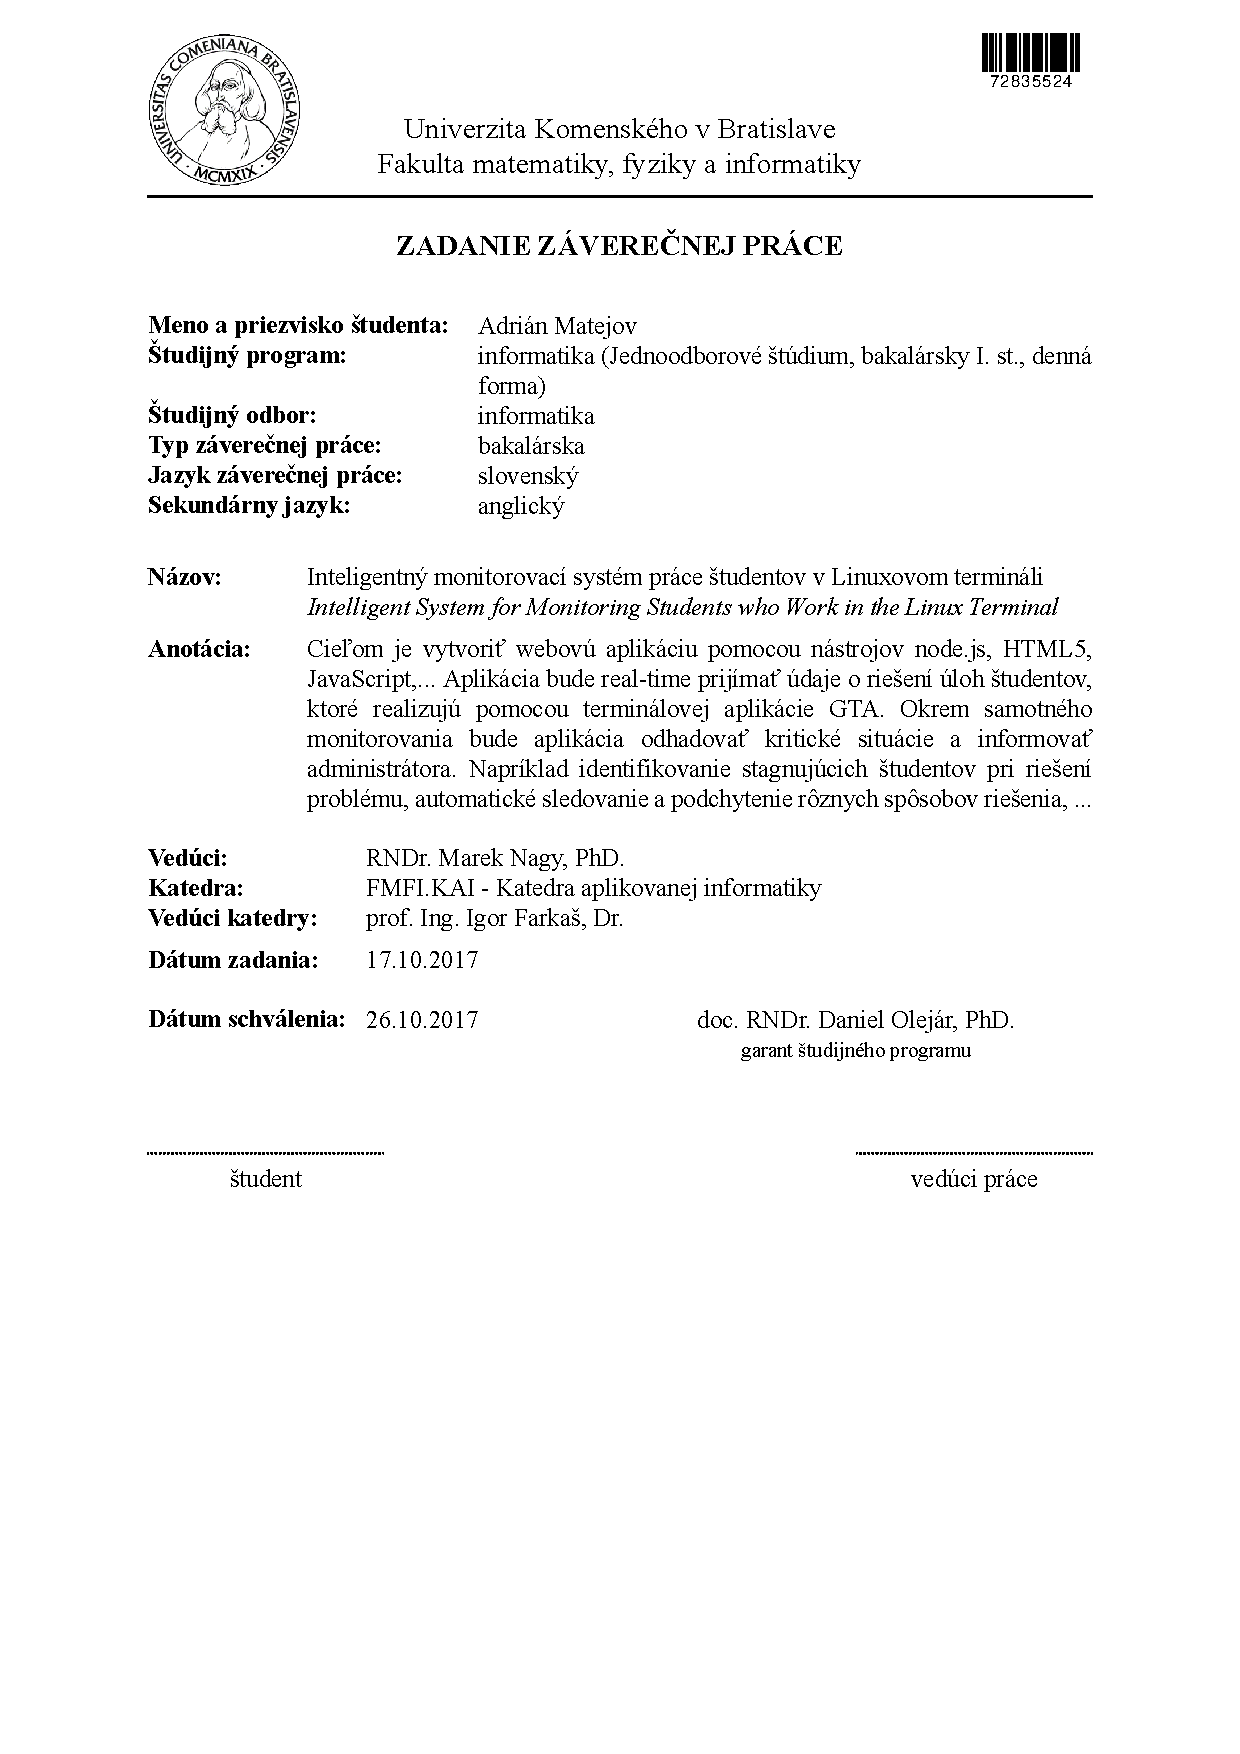
\includegraphics[width=1.1\textwidth]{images/zadanie}

% --- Koniec zadania

\frontmatter

% -------------------
%   Poďakovanie - nepovinné
% -------------------
\setcounter{page}{3}
\newpage 
~

\vfill
{\bf Poďakovanie:} Chcel by som sa poďakovať môjmu školiteľovi
RNDr. Marekovi Nagyovi, PhD. za poskytnuté konzultácie, cenné rady a možnosť
testovať systém na cvičeniach. Vďaka patrí Marekovi Šuppovi za mnoho nápadov, ochotu
diskutovať o vylepšeniach systému a pomoc s odosielaním dát.
Ďakujem aj mojej rodine a kamarátom, ktorí ma podporovali počas štúdia.

% --- Koniec poďakovania

% -------------------
%   Abstrakt - Slovensky
% -------------------
\newpage 
\section*{Abstrakt}


V tejto práci predstavujeme administratívny a monitorovací systém, ktorý slúži na
monitorovanie priebehu cvičenia, kde študenti pracujú v Linuxovom termináli.
Systém sa snaží automaticky detegovať neaktivitu alebo zaseknutie študentov
pri konkrétnych úlohách a okamžite upozorňovať vyučujúceho.
Takto dostáva učiteľ oveľa lepší prehľad o napredovaní študentov.
Po cvičení ponúka rozhranie na automatické ohodnotenie riešení a
detekciu rôznych spôsobov riešenia úloh pomocou metódy K-means.

\paragraph*{Kľúčové slová:} monitorovanie, webová aplikácia, Node.js, K-means
% --- Koniec Abstrakt - Slovensky


% -------------------
% --- Abstrakt - Anglicky 
% -------------------
\newpage 
\section*{Abstract}

This thesis introduces administrative and monitoring system for monitoring the course of
seminar,
where students work in the Linux terminal. The system automatically detects
inactivity of students or students being stuck on particular task
and immediately notifies the teacher about them.
This way the teacher has much better overview of progresses of students.
After the seminar, the system provides interface for automatically evaluating
assignments and detection of different ways of solving tasks using K-means method.

\paragraph*{Keywords:} monitoring, web application, Node.js, K-means

% --- Koniec Abstrakt - Anglicky


% -------------------
% --- Obsah
% -------------------

\newpage 

\tableofcontents

% ---  Koniec Obsahu

% -------------------
% --- Zoznamy tabuliek, obrázkov - nepovinne
% -------------------

\newpage 

\listoffigures
\listoftables

% ---  Koniec Zoznamov

\mainmatter


\input introduction.tex 

\input specifikacia.tex

\input navrh.tex

\input implementacia.tex

\input testovanie.tex

\input conclusion.tex

% -------------------
% --- Bibliografia
% -------------------


\newpage	

\backmatter

\thispagestyle{empty}
\nocite{*}
\clearpage

\bibliographystyle{plain}
\bibliography{literatura} 

%---koniec Referencii

% -------------------
%--- Prilohy---
% -------------------

%Nepovinná časť prílohy obsahuje materiály, ktoré neboli zaradené priamo  do textu. Každá príloha sa začína na novej strane.
%Zoznam príloh je súčasťou obsahu.
%
\input AppendixA.tex
\addcontentsline{toc}{chapter}{Appendix A}
%
%\addcontentsline{toc}{chapter}{Appendix B}
%\input AppendixB.tex

\end{document}
